\section{РЕАЛИЗАЦИЯ КЛИЕНТСКОЙ ЧАСТИ}

\subsection{Реализация функционала заполнения и сохранения карт вызова}

Функционал заполнения и сохранения карт вызова представляет собой важную часть медицинского приложения, которое позволяет медицинским работникам эффективно вести медицинскую документацию и сохранять данные о пациентах. Перед реализацией функционала заполнения, необходимо подробно рассмотреть обратную сторону карты вызова, рисунок~\ref{fig:medical-card} .Для удобства навигации и промежуточного сохранения заполненных полей карта вызова должна быть разделена на несколько разделов.

Первым является раздел  - "Жалобы и Анамнез" - предназначен для заполнения данных о жалобах пациента и его медицинском анамнезе. Здесь медицинский работник может внести подробности, симптомы и предыдущую медицинскую историю пациента.

Следующий раздел - "Объективно" - предназначен для ввода объективных данных, полученных в результате осмотра пациента. Здесь могут быть указаны физические параметры, результаты осмотра органов и систем пациента.

Затем идут разделы, посвященные различным системам органов, такие как "Органы Дыхания", "Органы кровообращения", "Органы Пищеварения", "Нервная Система", "Костная Система". В каждом из этих разделов можно внести подробности о соответствующей системе органов пациента, включая симптомы, результаты исследований и т.д.

В разделе "Status Localis" заполняются основные данные о пациенте, такие как вес, пол, рост, возраст. Эти данные могут быть переданы модулям "Калькулятор дозировок" и "Таблицы Дифференциальной диагностики" через инструмент Redux, чтобы обеспечить удобную работу с этими данными в указанных модулях.

В разделе "Данные инструментальных исследований" может быть реализована функция загрузки фотографии снимка ЭКГ. После загрузки фотографии она может быть отправлена на сервер для обработки модулем "Острые патологии по снимку ЭКГ". Это позволит медицинскому персоналу быстро анализировать и диагностировать патологии на основе снимков ЭКГ.

В разделе "Оказанная помощь, ее эффект и рекомендации" необходимо указать информацию о предоставленной медицинской помощи, ее результаты и рекомендации для пациента.

И, наконец, раздел "Расходные материалы" предназначен для внесения информации о расходных материалах, использованных при оказании медицинской помощи.

Каждый раздел имеет множество полей, которые заполняются медицинским работником в соответствии с конкретной ситуацией и состоянием пациента. Для обеспечения более быстрого заполнения карты вызова необходимо проанализировать заполненные поля уже заполненных карт и выявить часто встречающиеся ответы. На основе этого анализа необходимо реализовать дополнительный функционал быстрых ответов, который предложит предварительно заполненные часто используемые значения для данных полей, что значительно ускорит процесс заполнения карты вызова. Промежуточный результат разработки заполнения карты вызова можно увидеть на рисунке~\ref{fig:result1}

\begin{figure}
  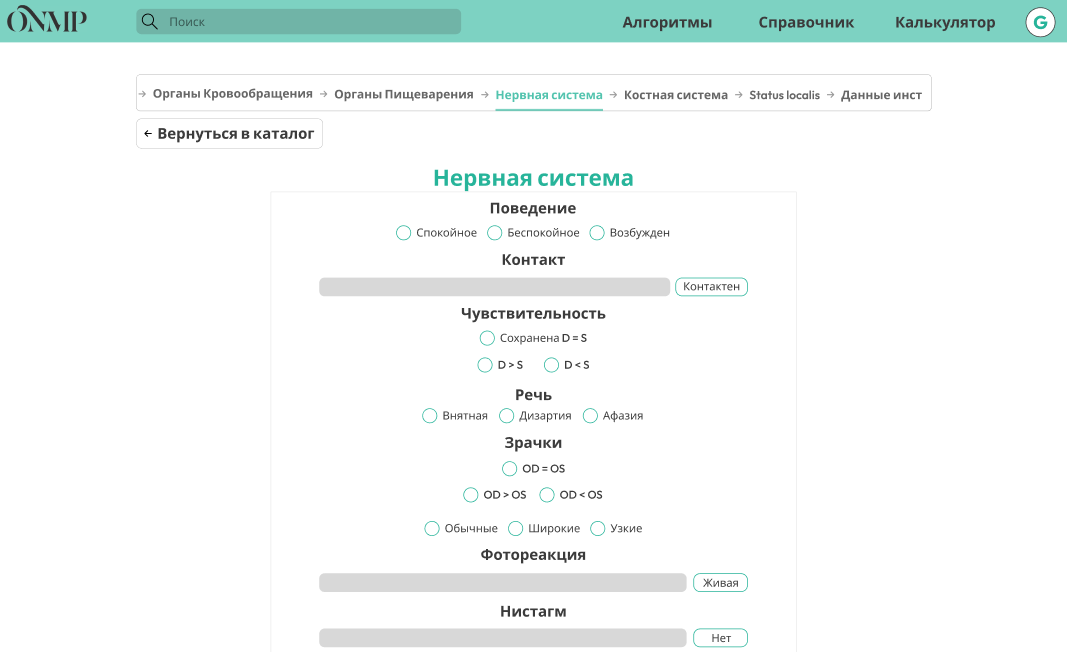
\includegraphics[scale=0.58]{styles/diploma/inc/result1.png}
  \caption{Страница заполнения карты вызова}
  \label{fig:result1}
\end{figure}

В результате реализации функционала заполнения и сохранения карт вызова в соответствии с описанными разделами, медицинские работники смогут эффективно и точно вести медицинскую документацию, сохранять данные о пациентах и облегчить себе работу при последующих визитах или обращениях пациентов.

\subsection{Разработка функционала организации папок и использования шаблонов}

Функционал организации папок и использования шаблонов для карт вызова обеспечивает максимальную эффективность и удобство использования. Разработка этого функционала включает создание четырех папок: Готовые, Незавершенные, Архив и Шаблоны.

В папку "Готовые" попадают карты вызова после того, как пользователь успешно заполнил все необходимые поля и нажал кнопку "Сохранить". Такая организация позволяет пользователям легко находить готовые карты вызова и быстро получать доступ к информации о каждом вызове.

В папку "Незавершенные" попадают карты вызова, когда пользователь не завершает их заполнение, например, закрывает вкладку или не нажимает кнопку "Сохранить". Однако уже введенные данные сохраняются в базе данных в процессе заполнения, чтобы пользователь мог возобновить работу с того места, где он остановился. Это обеспечивает сохранность введенных данных и позволяет избежать необходимости повторного заполнения всех полей.

В папку "Архив" перемещаются карты вызова после их распечатки или выполнения других действий, указанных пользователем. Архивирование карт вызова обеспечивает сохранность уже готовых карт, которые могут быть полезными для последующего анализа статистики, отчетов и других целей.

Папка "Шаблоны" предоставляет возможность создания базовых шаблонов карт вызова с частичным заполнением полей. Пользователи могут создавать шаблоны с предварительно заполненными данными, которые могут быть использованы в будущем как основа для создания новых карт вызова. Это существенно ускоряет процесс заполнения карт, поскольку многие поля уже будут заполнены заранее, и пользователю останется только внести дополнительную информацию. В результате, пользователи смогут более эффективно использовать время при заполнении карт вызова и уменьшить вероятность ошибок. Промежуточный результат разработки списка карт можно увидеть на рисунке~\ref{fig:result2}

\begin{figure}
  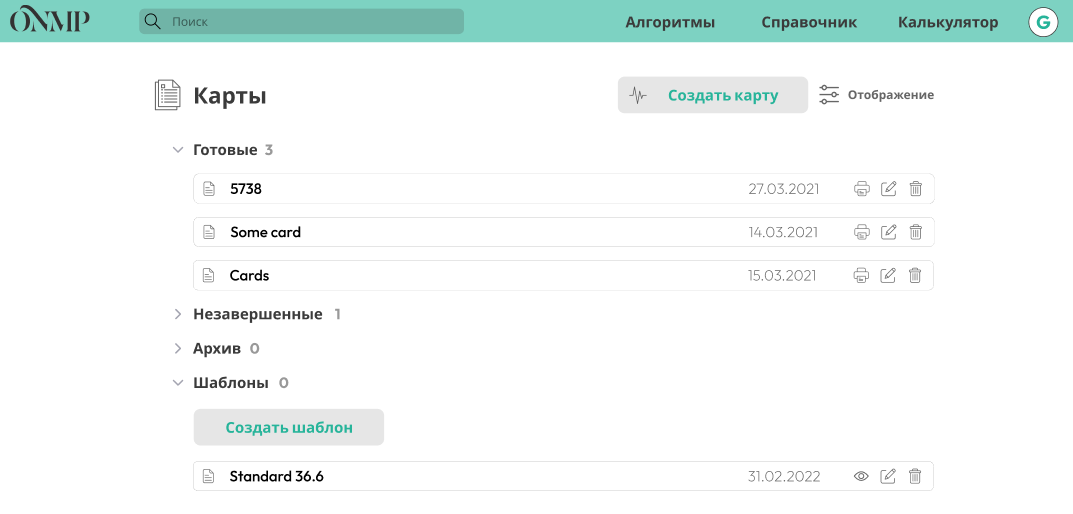
\includegraphics[scale=0.58]{styles/diploma/inc/result2.png}
  \caption{Страница со списком созданных карт}
  \label{fig:result2}
\end{figure}

Реализация функционала организации папок и шаблонов обеспечивает структурированный подход к хранению и управлению картами вызова, улучшает доступность и обработку данных, а также повышает эффективность работы с ними. Это существенно упрощает процесс работы медицинского персонала и повышает общую производительность системы.
